\section{Impact on Shear Systematics}

Systematics due to DCR affect the shapes of both stars and galaxies by biasing their PSF. 
The amount of bias is determined by the SED of the star or galaxy within the observing band.
Though this is correlated with colour, it propagates in (different) complex ways for stars and galaxies (See \citealt{meyersburchat15}).
We approximate this effect.
Considering only the colour difference between stars in the PSF model and galaxies (and not SEDs), we investigate the impact of this "mean-colour DCR error" on cosmic shear.
The errors due to this mean-colour DCR error are additive and can typically be represented as,

\begin{equation*}
    \gamma_{\rm obs} = \gamma_{\rm true}  + \beta \delta\mathbf{e}^{\rm DCR}
\end{equation*}

to second order, where $\beta$ is calculated from the rho-statistics and tau-statistics and quantifies the impact from PSF modeling error on shape modeling errors \cite[E.g.][]{gatti2021}]. Typically, $\beta$ is of order 1. Therefore, ignoring chance correlations $\langle \gamma_{\rm true} \delta\mathbf{e}^{\rm DCR}\rangle$, and choosing $\beta = 1$, the impact on the cosmic shear is approximately,

\begin{equation*}
    \langle \gamma_{\rm obs}\gamma_{\rm obs} \rangle \approx \langle \gamma_{\rm true}\gamma_{\rm true} \rangle  + \langle \delta\mathbf{e}^{\rm DCR} \delta\mathbf{e}^{\rm DCR}\rangle.
\end{equation*}

In practice, we can forecast this impact as follows.
As shown in Figure \ref{fig:g_dcr} \& \ref{fig:r_dcr}, the $\delta\mathbf{e}^{\rm DCR}$ due to DCR is determined empirically using a test set PSF star exposures reserved from the modeling. 
The values $\rm DCR_1$ and $\rm DCR_2$ themselves can also be determined from the time, RA and Dec of observation and through Equation \ref{eq:dcr}. 
From the LSST survey scheduler OpSim Baseline v5.1.0, we find this information for each exposure, calculate and tile the $\rm DCR$ values across the exposure field of view (approximated as a circle of radius 1.75\textdegree), and finally aggregate them into a HEALPix map of the sky weighted by the effective exposure time $T_{\rm eff}\times \rm visitExposureTime$.
This is shown in Figure \ref{fig:dcr_maps}.

\begin{figure}[h!]
    \centering
\includegraphics[width=0.9\textwidth]{figures/LSSTY10_DCR.png}
    \caption{Differential Chromatic Refraction maps for LSST Y10 WFD using OpSim Baseline v5.1.0.} 
    \label{fig:dcr_maps}
\end{figure}

The mean-colour DCR error is a function of the colour difference between the average PSF star and galaxies. Therefore, higher redshift galaxies that are redder have greater DCR effect. 
We estimate the average range of source galaxy colours in LSST redshift bins using galaxies from DES.
To do so, we draw galaxies from the DES into LSST redshift bins and use their colour distribution  for LSST.
Given that LSST goes to higher redshifts than DES, this works for all but the last redshift bin. 
For this bin, we linearly extrapolate the galaxy colours out to high redshift.
This assumption is likely the largest source of inaccuracy in the forecasts for this redshift bin (bin 5), as the slope of the $\rm{DCR}-\delta e$ relation itself is sensitive to the $\textit{r}-\textit{z}$ colour of the galaxies.
Additionally, as the Balmer break shifts out of the {\it z} band at $z\approx 1.5$, it is unlikely that the galaxy colours increase linearly.
However, for a worst-case forecast, this is a reasonable assumption.

\begin{figure}[h!]
    \centering
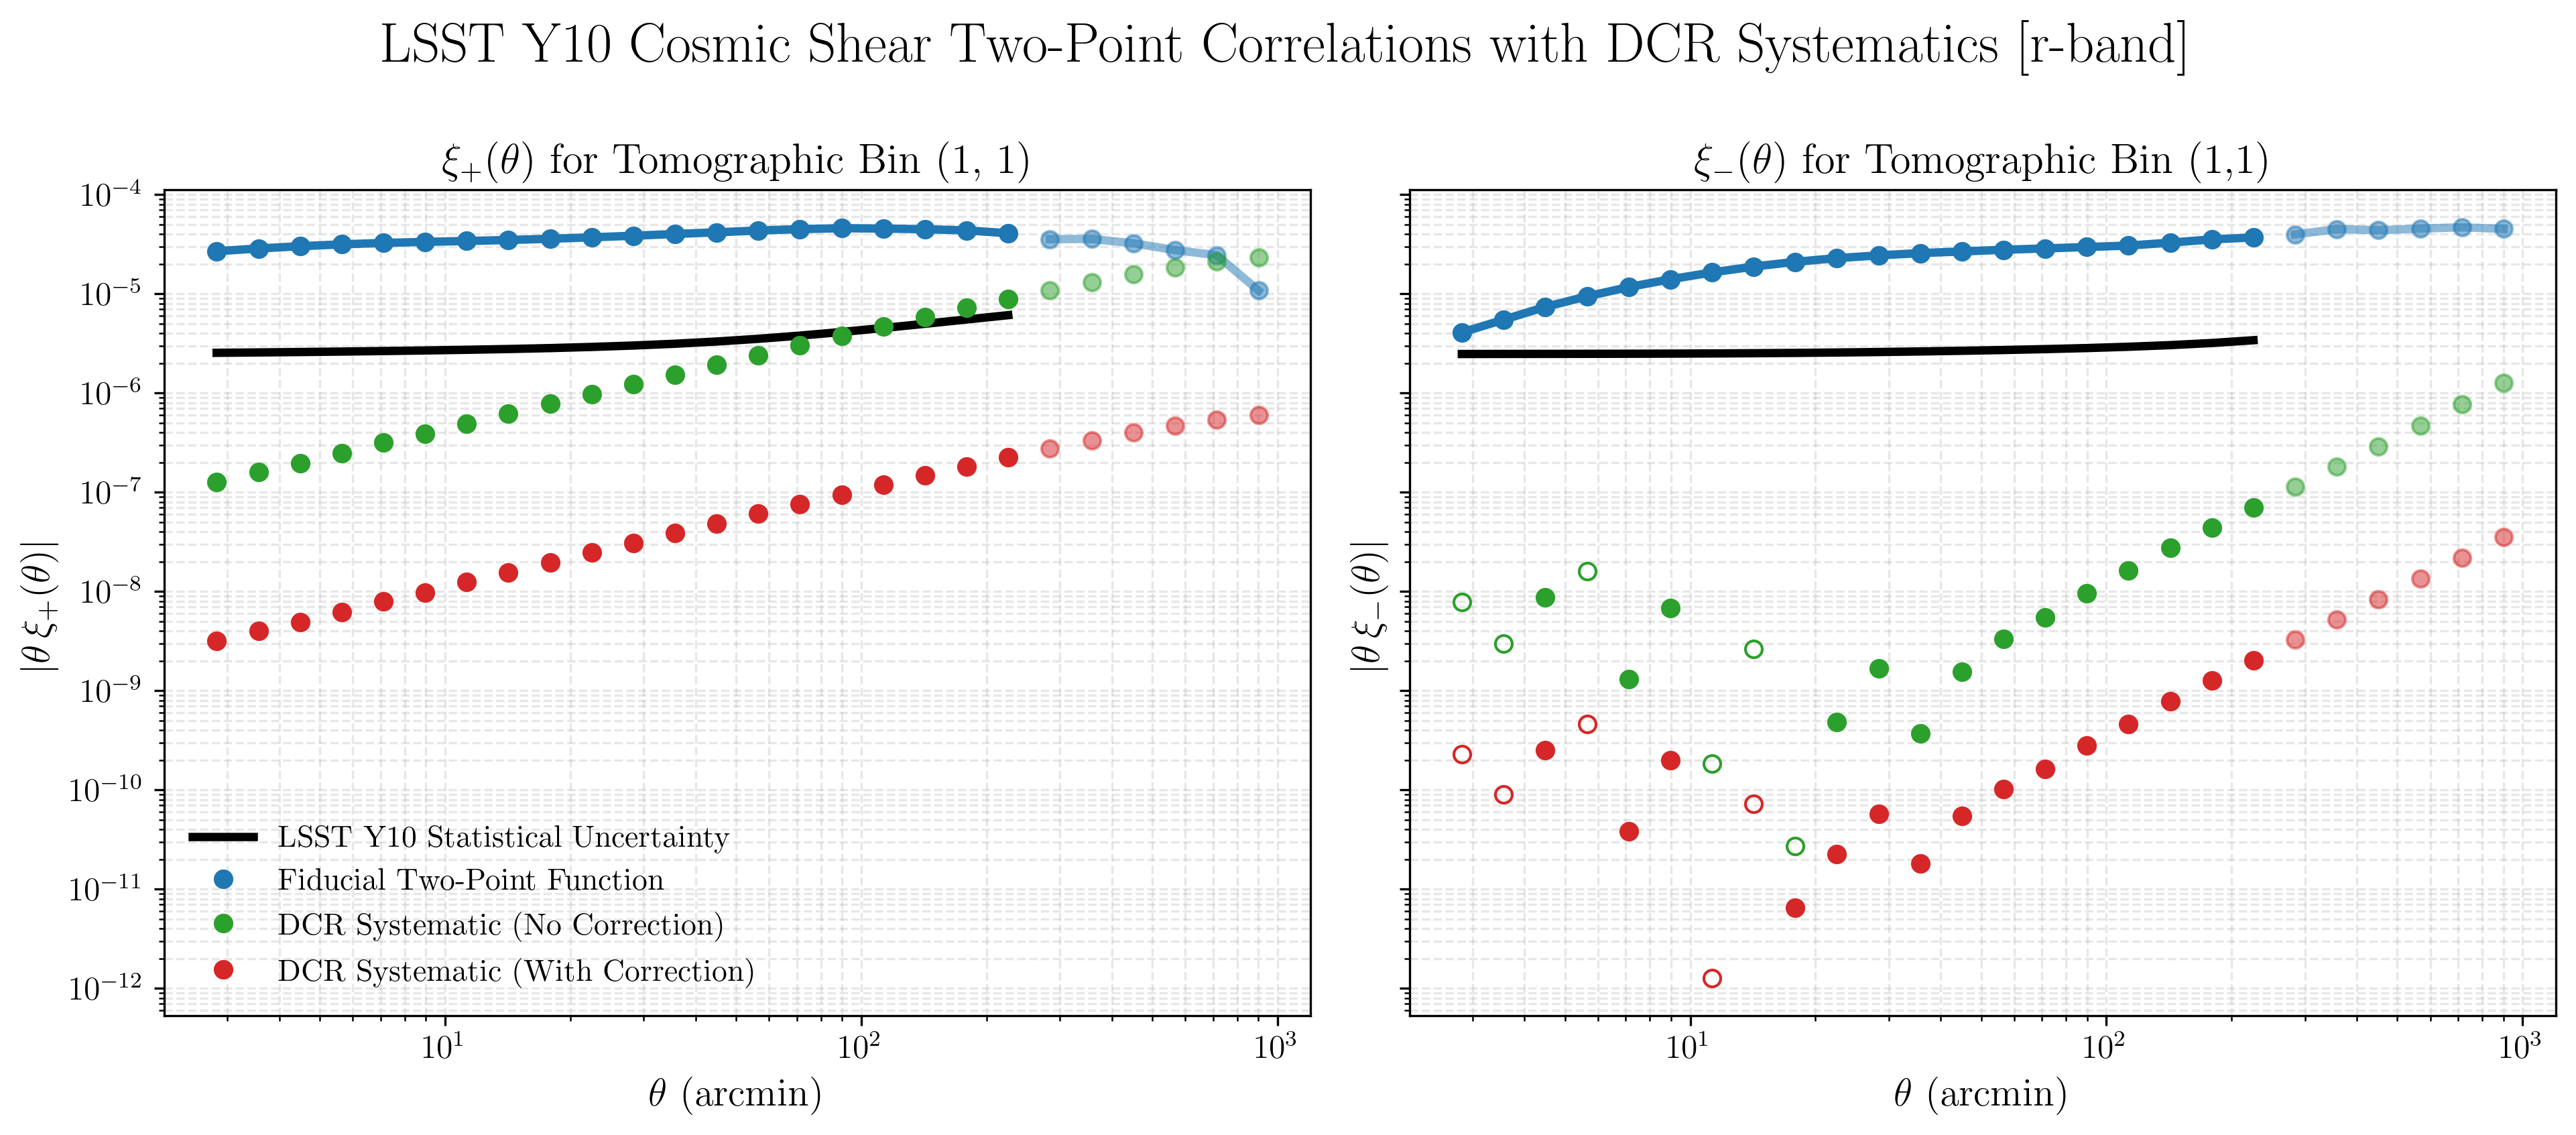
\includegraphics[width=0.9\textwidth]{figures/LSSTY10_dcrsyst_11r.png}
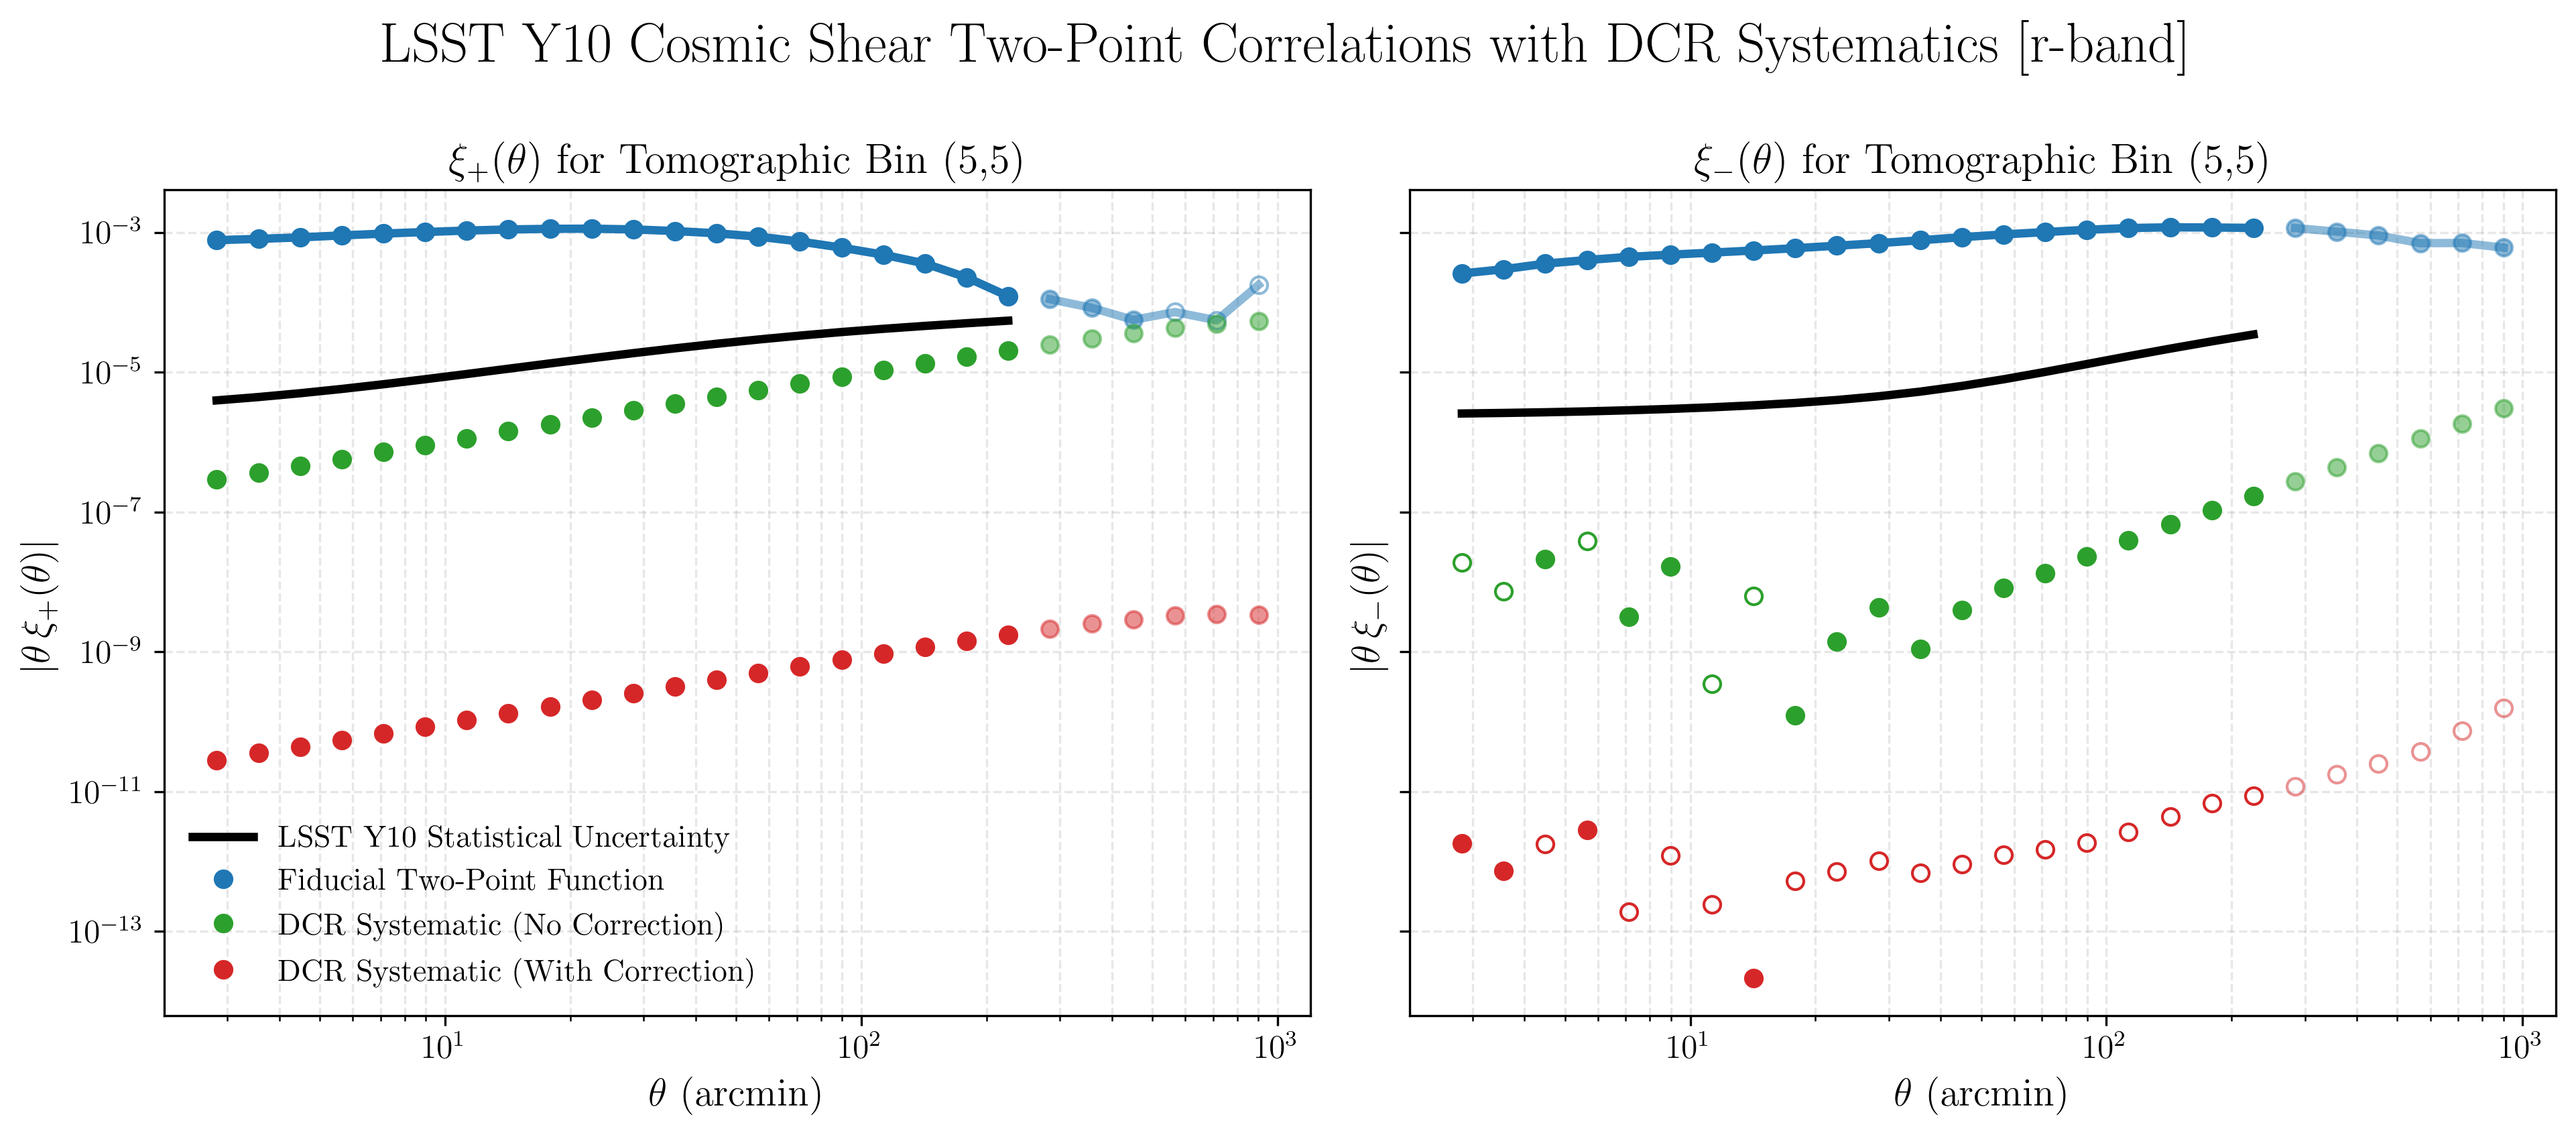
\includegraphics[width=0.9\textwidth]{figures/LSSTY10_dcrsyst_55r.png}
    \caption{Impact of mean-colour DCR error on the cosmic shear two-point correlation function, for {\it r} band PSF exposures. In blue, we show the fiducial cosmic shear for the closest and furthest tomographic bin autocorrelation (1, 1) and bin (5, 5). The black line represents the uncertainty of cosmic shear from analytic covariance, for comparison. Data points beyond the DES cosmology range are faded. The DCR Systematic $\langle \delta\mathbf{e}^{\rm DCR} \delta\mathbf{e}^{\rm DCR}\rangle$ if uncorrected (shown in green) is below LSST Y10 statistical uncertainty for $\xi_+$ and $\xi_-$. The corrected DCR signal shown in red sufficiently reduces this effect by four orders of magnitude.} 
    \label{fig:dcr_syst}
\end{figure}

\begin{figure}[h!]
    \centering
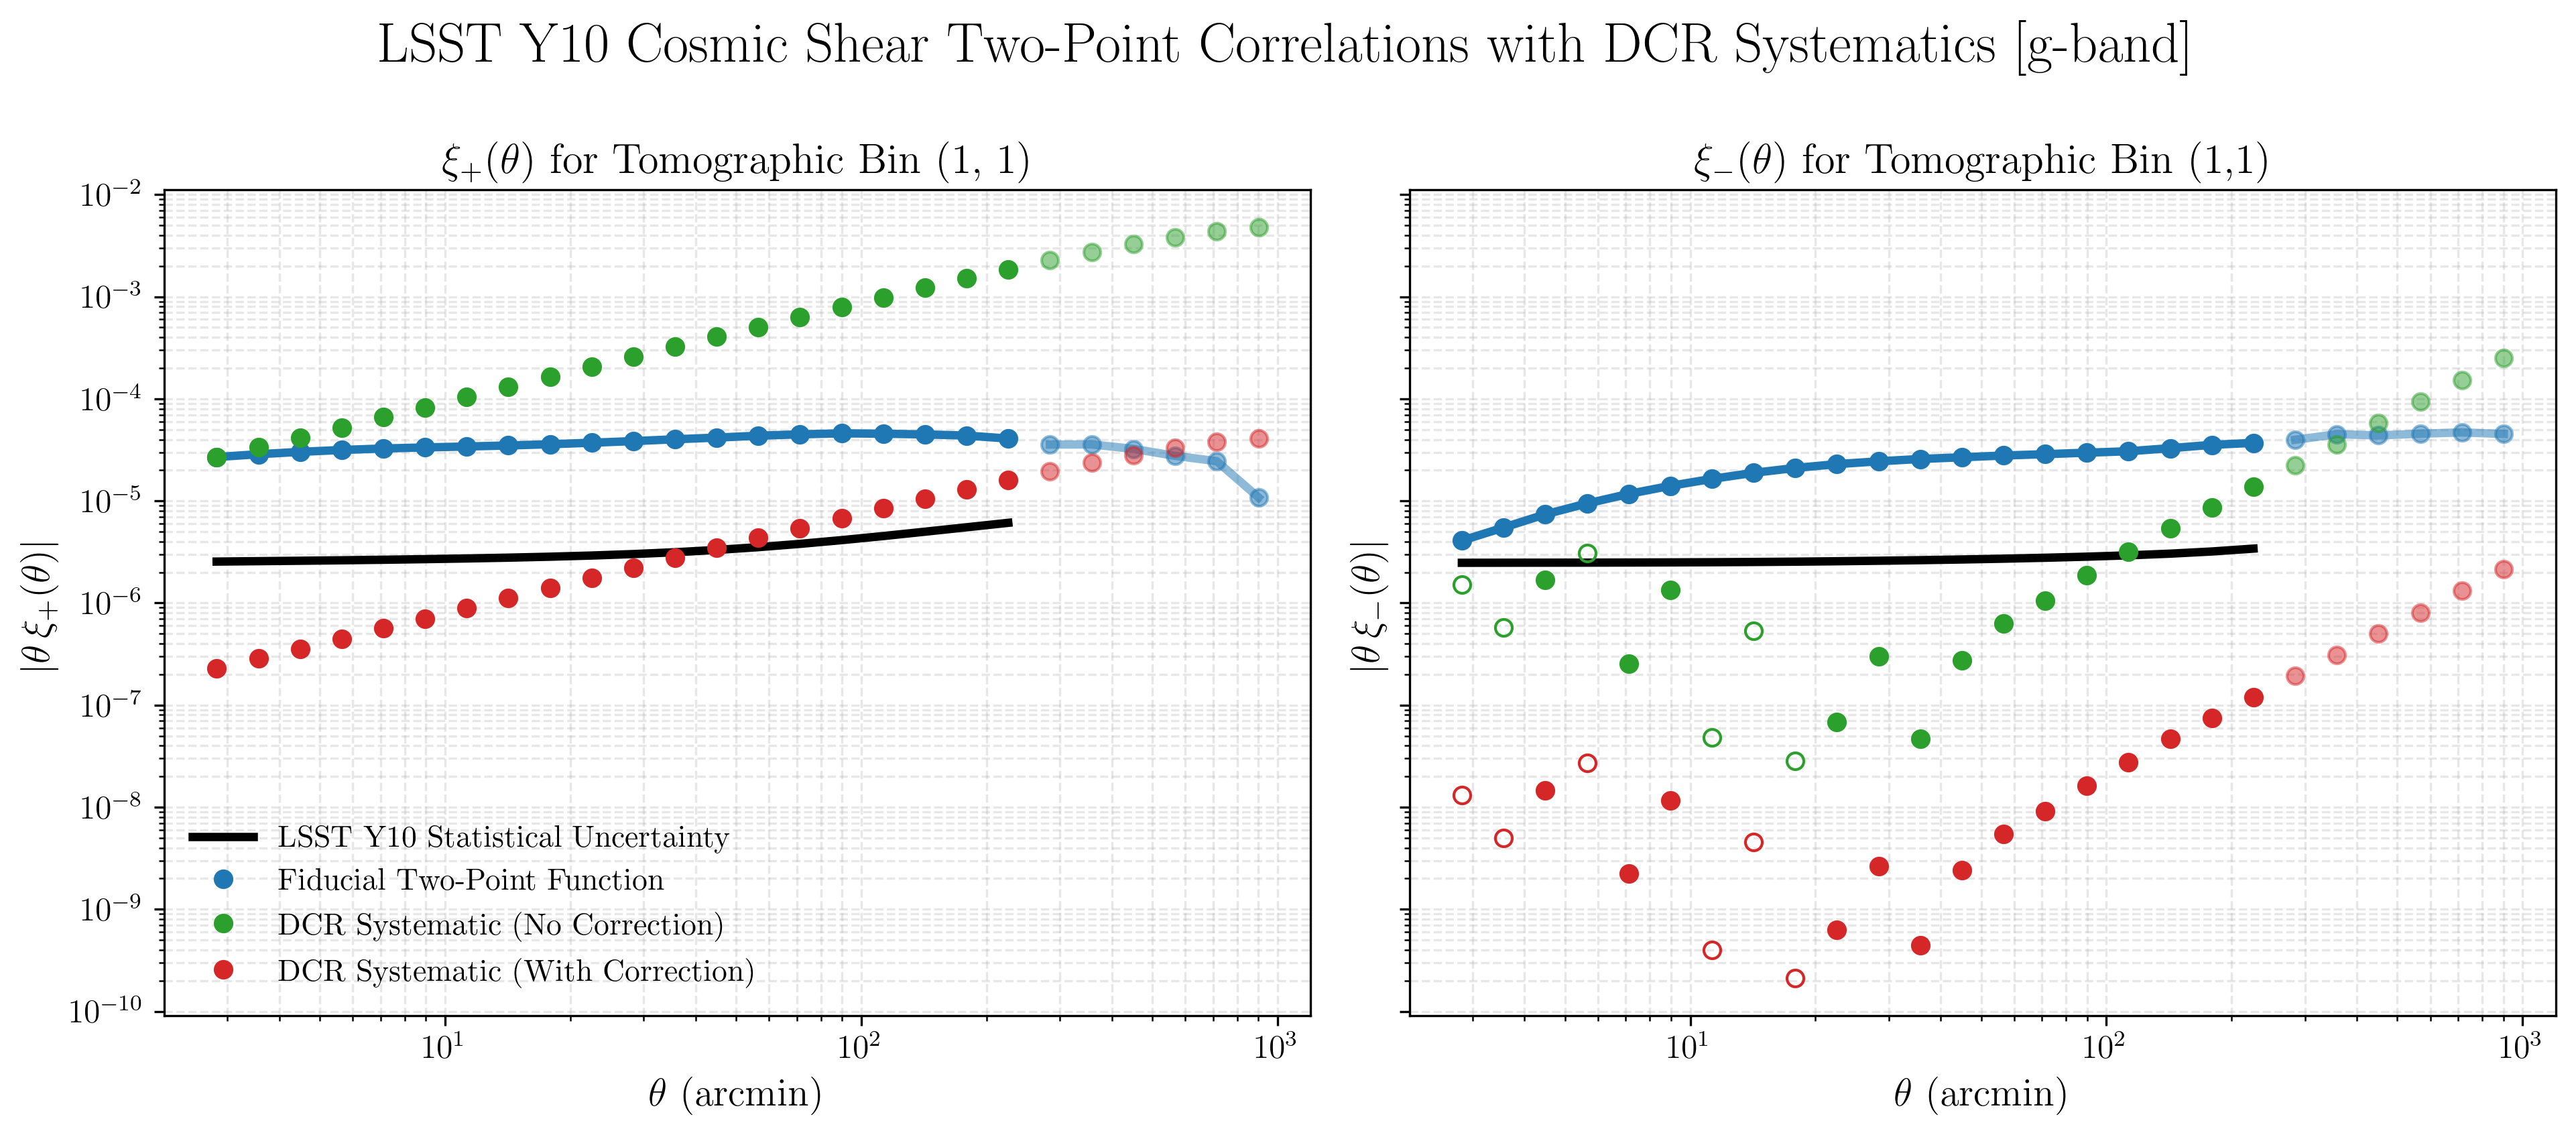
\includegraphics[width=0.9\textwidth]{figures/LSSTY10_dcrsyst_11g.png}
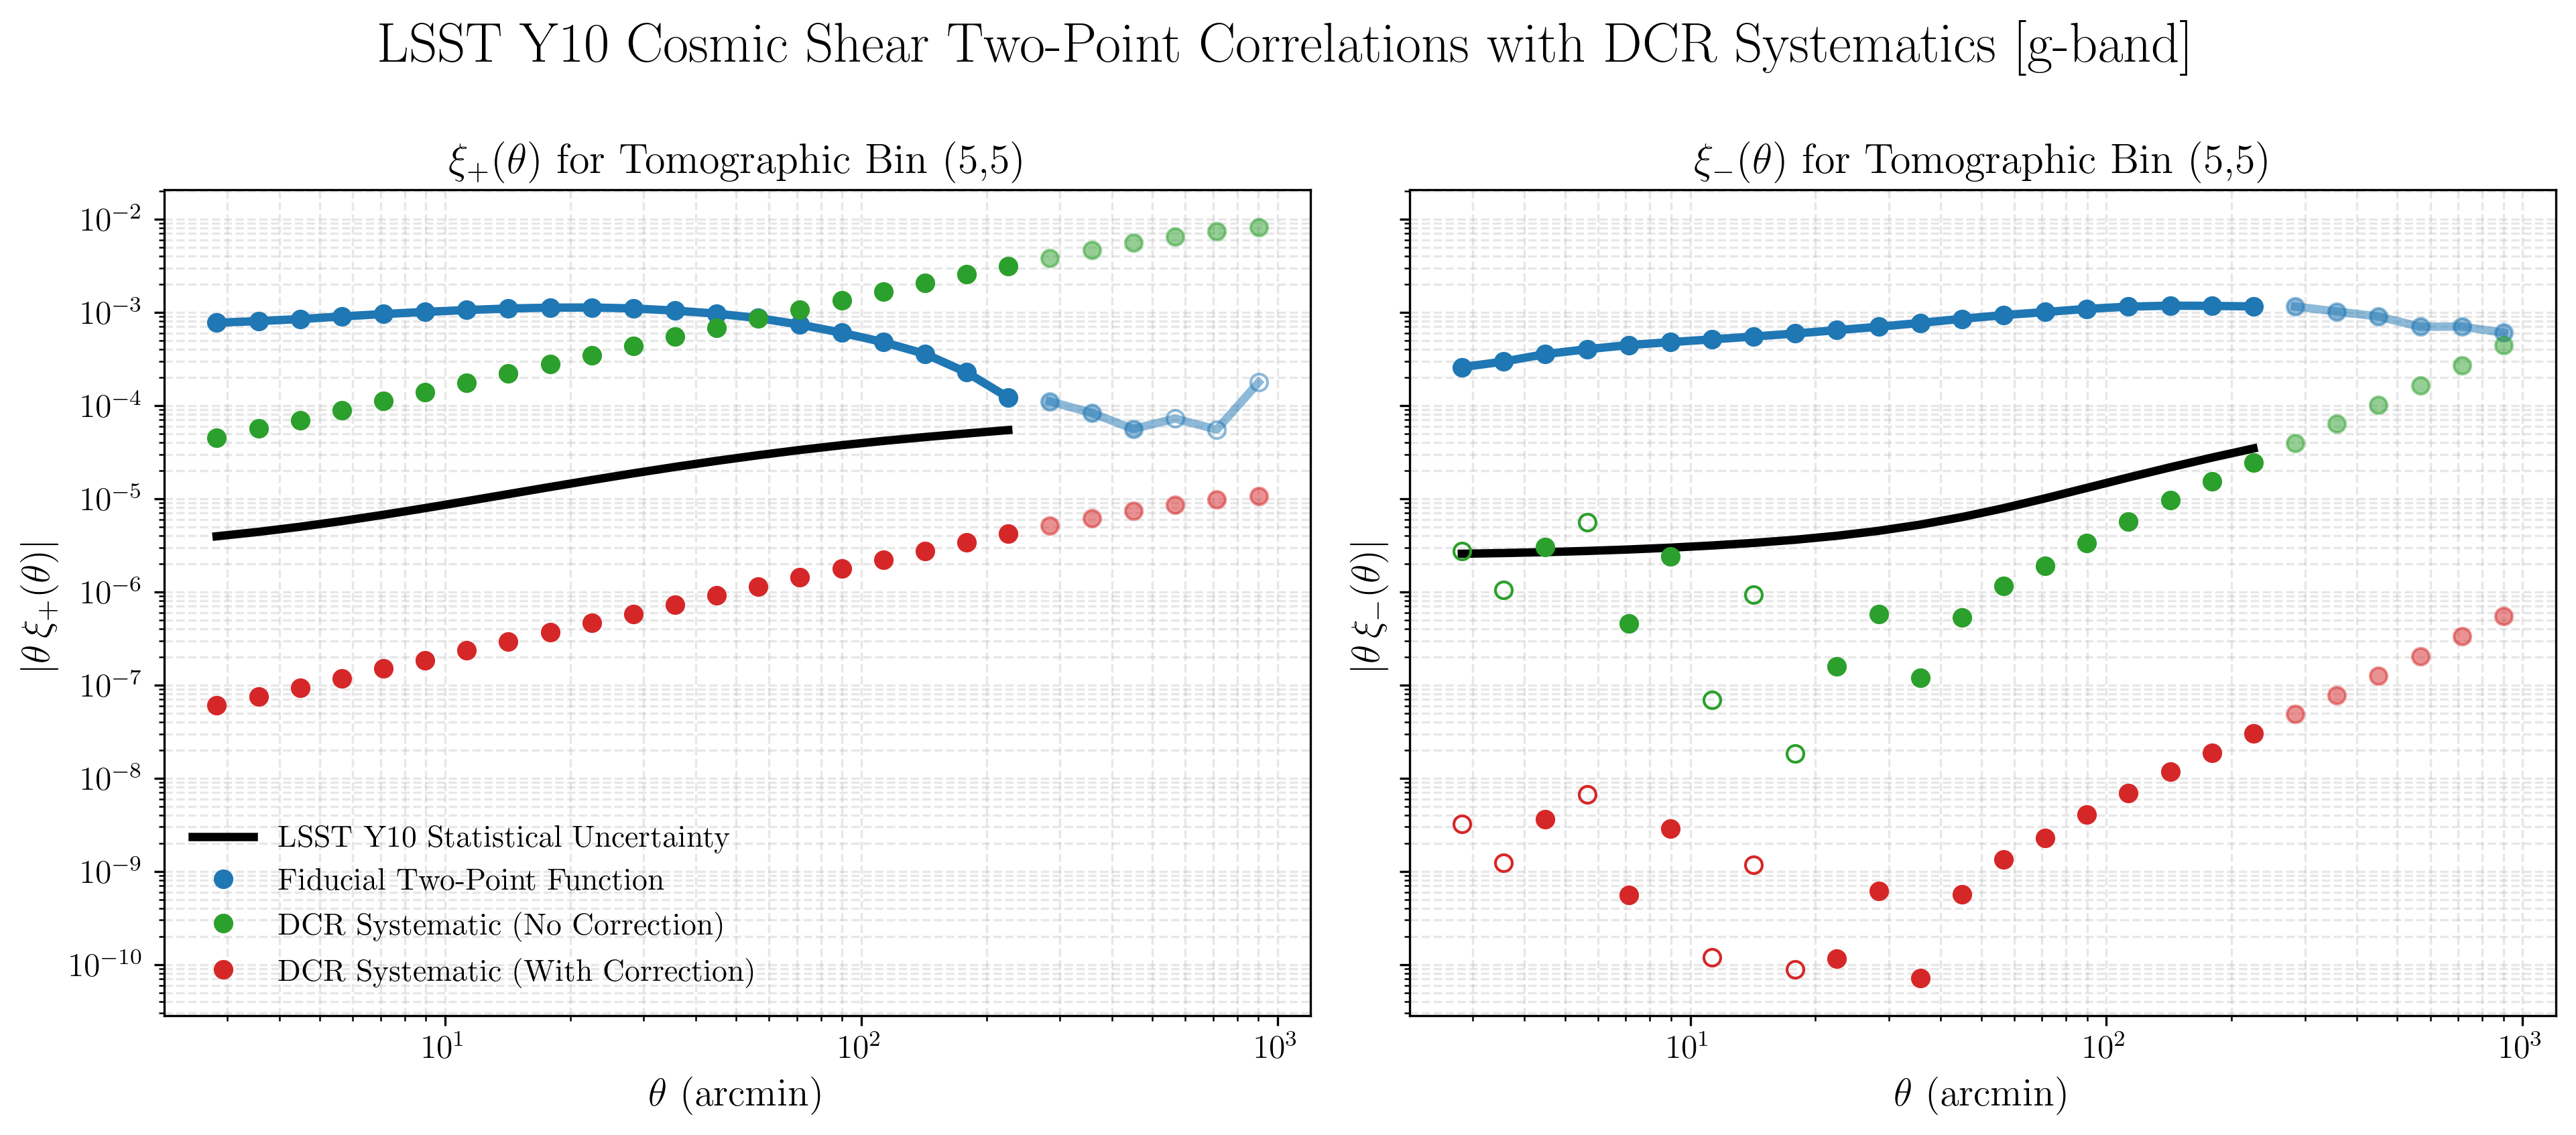
\includegraphics[width=0.9\textwidth]{figures/LSSTY10_dcrsyst_55g.png}
    \caption{Impact of mean-colour DCR error on the cosmic shear two-point correlation function, for the poorer {\it g} band PSF exposures. See Figure \ref{fig:dcr_syst} for format. The DCR Systematic $\langle \delta\mathbf{e}^{\rm DCR} \delta\mathbf{e}^{\rm DCR}\rangle$ if uncorrected (shown in green) will dominate the cosmic shear signal for $\xi_+$ and even bias $\xi_-$ if only uncorrected {\it g} band exposures are used. The corrected DCR signal shown in red reduces this effect, but may still impact bin (1, 1) at scales $\theta > 50 \, \rm arcmin$.} 
    \label{fig:dcr_syst_g}
\end{figure}

Finally, we linearly fit the colour-dependent $\rm{DCR}-\delta e$ relation for the uncorrected and corrected chromatic PSF case, and apply it to the DCR maps (Figure \ref{fig:dcr_maps}). 
To calculate the two-point correlation function of this error map, we use the \texttt{treecorr} software \citep{Jarvis2004}. 
We create a catalog from pixels, and perform the correlation $\langle \delta\mathbf{e}^{\rm DCR} \delta\mathbf{e}^{\rm DCR}\rangle$ for a range from 2.5 to 1000 arcmin, with 26 bins (to mimic DES within its range), and a \texttt{bin\_slop} of 0.1.
To forecast the shear signal and uncertainty, we use \texttt{GLASS} \citep{tessore2023}, alongside the redshift distributions forecast by the LSST Science Requirements Document \citep{lsstsrd2018} and \texttt{CosmoCov} \citep{krause2017, fang2020a} to estimate the analytic uncertainty. These results are shown in Figure \ref{fig:dcr_syst} for {\it r} band exposures and Figure \ref{fig:dcr_syst_g} for {\it g} band exposures.

We find that the mean-colour DCR systematic indeed has a non-negligible impact on $\xi_+$ when considering the better {\it r} band exposures, where for Y10 of the LSST survey, systematic uncertainties would have been on the level of statistical uncertainties for the (1, 1) tomographic bin correlation on large scales $\theta > 50 \,  \rm arcmin$. 
Correcting for the chromatic PSF using PiFF colour-dependence sufficiently reduces this systematic by four orders of magnitude.
Post-correction, on all scales, mean-colour DCR effects in {\it r} band remain subdominant to statistical errors.

The mean-colour DCR systematic on {\it g} band exposures, however, is significant. 
Uncorrected, for $\xi_+$ the error is on the order of the cosmic shear signal itself.
For $\xi_-$, the error is on the order of statistical uncertainties for small and large scales.
Post-correction, though the systematic is reduced by two to three orders of magnitude, the systematic error remains high for the (1, 1) autocorrelation on scales $\theta \gtrsim 50$.
This can be directly attributed to the order of magnitude higher DCR error in {\it g} band in the $\rm{DCR}-\delta e$ relation (Compare figures \ref{fig:g_dcr} \& \ref{fig:r_dcr}).
Given this, it is not recommended to use {\it g} band, similar to DES \citep{jarvis2021, schutt2025}, for which the {\it g} band error is similarly an order of magnitude above {\it r} band errors (Figure \ref{fig:des_dcr}).

Further detailed study of the forecasted impact of DCR and other shape systematics for LSST will be presented in  \citet{Agarwal2026}. 